% ARTICLE ----
% This is just here so I know exactly what I'm looking at in Rstudio when messing with stuff.
\documentclass[11pt,]{article}
\usepackage[left=1in,top=1in,right=1in,bottom=1in]{geometry}
\newcommand*{\authorfont}{\fontfamily{phv}\selectfont}
\usepackage[]{mathpazo}


  \usepackage[T1]{fontenc}
  \usepackage[utf8]{inputenc}




\usepackage{abstract}
\renewcommand{\abstractname}{}    % clear the title
\renewcommand{\absnamepos}{empty} % originally center

\renewenvironment{abstract}
 {{%
    \setlength{\leftmargin}{0mm}
    \setlength{\rightmargin}{\leftmargin}%
  }%
  \relax}
 {\endlist}

\makeatletter
\def\@maketitle{%
  \newpage
%  \null
%  \vskip 2em%
%  \begin{center}%
  \let \footnote \thanks
    {\fontsize{18}{20}\selectfont\raggedright  \setlength{\parindent}{0pt} \@title \par}%
}
%\fi
\makeatother




\setcounter{secnumdepth}{0}

\usepackage{color}
\usepackage{fancyvrb}
\newcommand{\VerbBar}{|}
\newcommand{\VERB}{\Verb[commandchars=\\\{\}]}
\DefineVerbatimEnvironment{Highlighting}{Verbatim}{commandchars=\\\{\}}
% Add ',fontsize=\small' for more characters per line
\usepackage{framed}
\definecolor{shadecolor}{RGB}{248,248,248}
\newenvironment{Shaded}{\begin{snugshade}}{\end{snugshade}}
\newcommand{\AlertTok}[1]{\textcolor[rgb]{0.94,0.16,0.16}{#1}}
\newcommand{\AnnotationTok}[1]{\textcolor[rgb]{0.56,0.35,0.01}{\textbf{\textit{#1}}}}
\newcommand{\AttributeTok}[1]{\textcolor[rgb]{0.13,0.29,0.53}{#1}}
\newcommand{\BaseNTok}[1]{\textcolor[rgb]{0.00,0.00,0.81}{#1}}
\newcommand{\BuiltInTok}[1]{#1}
\newcommand{\CharTok}[1]{\textcolor[rgb]{0.31,0.60,0.02}{#1}}
\newcommand{\CommentTok}[1]{\textcolor[rgb]{0.56,0.35,0.01}{\textit{#1}}}
\newcommand{\CommentVarTok}[1]{\textcolor[rgb]{0.56,0.35,0.01}{\textbf{\textit{#1}}}}
\newcommand{\ConstantTok}[1]{\textcolor[rgb]{0.56,0.35,0.01}{#1}}
\newcommand{\ControlFlowTok}[1]{\textcolor[rgb]{0.13,0.29,0.53}{\textbf{#1}}}
\newcommand{\DataTypeTok}[1]{\textcolor[rgb]{0.13,0.29,0.53}{#1}}
\newcommand{\DecValTok}[1]{\textcolor[rgb]{0.00,0.00,0.81}{#1}}
\newcommand{\DocumentationTok}[1]{\textcolor[rgb]{0.56,0.35,0.01}{\textbf{\textit{#1}}}}
\newcommand{\ErrorTok}[1]{\textcolor[rgb]{0.64,0.00,0.00}{\textbf{#1}}}
\newcommand{\ExtensionTok}[1]{#1}
\newcommand{\FloatTok}[1]{\textcolor[rgb]{0.00,0.00,0.81}{#1}}
\newcommand{\FunctionTok}[1]{\textcolor[rgb]{0.13,0.29,0.53}{\textbf{#1}}}
\newcommand{\ImportTok}[1]{#1}
\newcommand{\InformationTok}[1]{\textcolor[rgb]{0.56,0.35,0.01}{\textbf{\textit{#1}}}}
\newcommand{\KeywordTok}[1]{\textcolor[rgb]{0.13,0.29,0.53}{\textbf{#1}}}
\newcommand{\NormalTok}[1]{#1}
\newcommand{\OperatorTok}[1]{\textcolor[rgb]{0.81,0.36,0.00}{\textbf{#1}}}
\newcommand{\OtherTok}[1]{\textcolor[rgb]{0.56,0.35,0.01}{#1}}
\newcommand{\PreprocessorTok}[1]{\textcolor[rgb]{0.56,0.35,0.01}{\textit{#1}}}
\newcommand{\RegionMarkerTok}[1]{#1}
\newcommand{\SpecialCharTok}[1]{\textcolor[rgb]{0.81,0.36,0.00}{\textbf{#1}}}
\newcommand{\SpecialStringTok}[1]{\textcolor[rgb]{0.31,0.60,0.02}{#1}}
\newcommand{\StringTok}[1]{\textcolor[rgb]{0.31,0.60,0.02}{#1}}
\newcommand{\VariableTok}[1]{\textcolor[rgb]{0.00,0.00,0.00}{#1}}
\newcommand{\VerbatimStringTok}[1]{\textcolor[rgb]{0.31,0.60,0.02}{#1}}
\newcommand{\WarningTok}[1]{\textcolor[rgb]{0.56,0.35,0.01}{\textbf{\textit{#1}}}}



\title{Mood-Based Song Classifier. \thanks{Replication files are
available on the author's Github account
(\url{https://github.com/AlvaroNovillo/music_mood}). \textbf{Current
version}: febrero 20, 2024; \textbf{Corresponding author}:
\href{mailto:novillocorreasalvaro@gmail.com}{\nolinkurl{novillocorreasalvaro@gmail.com}}.}  }



\author{\Large Álvaro Novillo
Correas\vspace{0.05in} \newline\normalsize\emph{Universidad Carlos
III}  }


\date{}

\usepackage{titlesec}

\titleformat*{\section}{\normalsize\bfseries}
\titleformat*{\subsection}{\normalsize\itshape}
\titleformat*{\subsubsection}{\normalsize\itshape}
\titleformat*{\paragraph}{\normalsize\itshape}
\titleformat*{\subparagraph}{\normalsize\itshape}


\usepackage{natbib}
\bibliographystyle{apsr}
\usepackage[strings]{underscore} % protect underscores in most circumstances



\newtheorem{hypothesis}{Hypothesis}
\usepackage{setspace}


% set default figure placement to htbp
\makeatletter
\def\fps@figure{htbp}
\makeatother

\usepackage{graphicx}
\usepackage{hyperref}
\usepackage{float}
\usepackage{booktabs}
\usepackage{longtable}
\usepackage{array}
\usepackage{multirow}
\usepackage{wrapfig}
\usepackage{colortbl}
\usepackage{pdflscape}
\usepackage{tabu}
\usepackage{threeparttable}
\usepackage{threeparttablex}
\usepackage[normalem]{ulem}
\usepackage{makecell}
\usepackage{xcolor}

% move the hyperref stuff down here, after header-includes, to allow for - \usepackage{hyperref}

\makeatletter
\@ifpackageloaded{hyperref}{}{%
\ifxetex
  \PassOptionsToPackage{hyphens}{url}\usepackage[setpagesize=false, % page size defined by xetex
              unicode=false, % unicode breaks when used with xetex
              xetex]{hyperref}
\else
  \PassOptionsToPackage{hyphens}{url}\usepackage[draft,unicode=true]{hyperref}
\fi
}

\@ifpackageloaded{color}{
    \PassOptionsToPackage{usenames,dvipsnames}{color}
}{%
    \usepackage[usenames,dvipsnames]{color}
}
\makeatother
\hypersetup{breaklinks=true,
            bookmarks=true,
            pdfauthor={Álvaro Novillo Correas (Universidad Carlos III)},
             pdfkeywords = {pandoc, r markdown, knitr},
            pdftitle={Mood-Based Song Classifier.},
            colorlinks=true,
            citecolor=blue,
            urlcolor=blue,
            linkcolor=magenta,
            pdfborder={0 0 0}}
\urlstyle{same}  % don't use monospace font for urls

% Add an option for endnotes. -----


% add tightlist ----------
\providecommand{\tightlist}{%
\setlength{\itemsep}{0pt}\setlength{\parskip}{0pt}}

% add some other packages ----------

% \usepackage{multicol}
% This should regulate where figures float
% See: https://tex.stackexchange.com/questions/2275/keeping-tables-figures-close-to-where-they-are-mentioned
\usepackage[section]{placeins}

% CSL environment change -----


% Last minute stuff -----
\usepackage{amssymb,amsmath} % HT @ashenkin


\begin{document}

% \pagenumbering{arabic}% resets `page` counter to 1
%
% \maketitle

{% \usefont{T1}{pnc}{m}{n}
\setlength{\parindent}{0pt}
\thispagestyle{plain}
{\fontsize{18}{20}\selectfont\raggedright
\maketitle  % title \par

}

{
   \vskip 13.5pt\relax \normalsize\fontsize{11}{12}
\textbf{\authorfont Álvaro Novillo
Correas} \hskip 15pt \emph{\small Universidad Carlos III}   

}

}








\begin{abstract}

    \hbox{\vrule height .2pt width 39.14pc}

    \vskip 8.5pt % \small

\noindent In this article, following a similar procedure to
\citep{data1}, we apply several machine learning techniques to classify
songs into four different moods: energetic, happy, calm and sad. We then
implement a Shiny app that uses Python to scrape data from Spotify,
given an artist name or playlist URL, and perform an analysis of the
different characteristics and emotions that the artist's discography or
playlist has.


\vskip 8.5pt \noindent \emph{Keywords}: pandoc, r markdown, knitr \par

    \hbox{\vrule height .2pt width 39.14pc}



\end{abstract}


\vskip -8.5pt


 % removetitleabstract

\noindent 

\hypertarget{introduction.}{%
\section{Introduction.}\label{introduction.}}

Music, among other art forms, has an special ability to evoke emotions,
shaping our experiences and perceptions. In this article, we will delve
into the intricate relationship between music and emotions, using
machine learning techniques to analyze and categorize songs based on
their emotional content.

Building on previous research \citep{data1}, we will classify songs into
four primary emotional categories: energetic, happy, calm, and sad. To
achieve this, we'll leverage a dataset\footnote{1} of 686 previously
classified songs and develop a robust model capable of discerning the
encoded emotionality within musical compositions.

\begin{table}[!h]

\caption{\label{tab:unnamed-chunk-1}Pre-classified dataset used to train the model}
\centering
\resizebox{\linewidth}{!}{
\begin{tabular}[t]{llllrrrrrrrrrl}
\toprule
name & artist & album & id & danceability & acousticness & energy & instrumentalness & liveness & valence & loudness & speechiness & tempo & mood\\
\midrule
\cellcolor{gray!6}{1999} & \cellcolor{gray!6}{Prince} & \cellcolor{gray!6}{1999} & \cellcolor{gray!6}{2H7PHVdQ3mXqEHXcvclTB0} & \cellcolor{gray!6}{0.866} & \cellcolor{gray!6}{0.13700} & \cellcolor{gray!6}{0.7300} & \cellcolor{gray!6}{0.00e+00} & \cellcolor{gray!6}{0.0843} & \cellcolor{gray!6}{0.625} & \cellcolor{gray!6}{-8.201} & \cellcolor{gray!6}{0.0767} & \cellcolor{gray!6}{118.523} & \cellcolor{gray!6}{Happy}\\
23 & Blonde Redhead & 23 & 4HIwL9ii9CcXpTOTzMq0MP & 0.381 & 0.01890 & 0.8320 & 1.96e-01 & 0.1530 & 0.166 & -5.069 & 0.0492 & 120.255 & Sad\\
\cellcolor{gray!6}{9 Crimes} & \cellcolor{gray!6}{Damien Rice} & \cellcolor{gray!6}{9} & \cellcolor{gray!6}{5GZEeowhvSieFDiR8fQ2im} & \cellcolor{gray!6}{0.346} & \cellcolor{gray!6}{0.91300} & \cellcolor{gray!6}{0.1390} & \cellcolor{gray!6}{7.73e-05} & \cellcolor{gray!6}{0.0934} & \cellcolor{gray!6}{0.116} & \cellcolor{gray!6}{-15.326} & \cellcolor{gray!6}{0.0321} & \cellcolor{gray!6}{136.168} & \cellcolor{gray!6}{Sad}\\
99 Luftballons & Nena & 99 Luftballons & 6HA97v4wEGQ5TUClRM0XLc & 0.466 & 0.08900 & 0.4380 & 5.60e-06 & 0.1130 & 0.587 & -12.858 & 0.0608 & 193.100 & Happy\\
\cellcolor{gray!6}{A Boy Brushed Red Living In Black And White} & \cellcolor{gray!6}{Underoath} & \cellcolor{gray!6}{They're Only Chasing Safety} & \cellcolor{gray!6}{47IWLfIKOKhFnz1FUEUIkE} & \cellcolor{gray!6}{0.419} & \cellcolor{gray!6}{0.00171} & \cellcolor{gray!6}{0.9320} & \cellcolor{gray!6}{0.00e+00} & \cellcolor{gray!6}{0.1370} & \cellcolor{gray!6}{0.445} & \cellcolor{gray!6}{-3.604} & \cellcolor{gray!6}{0.1060} & \cellcolor{gray!6}{169.881} & \cellcolor{gray!6}{Energetic}\\
\addlinespace
A Burden to Bear & Emmanuelle Rimbaud & A Burden to Bear & 67DOFCrkcQaLp5yhzF8Y8N & 0.394 & 0.99500 & 0.0475 & 9.55e-01 & 0.1050 & 0.172 & -26.432 & 0.0720 & 71.241 & Calm\\
\bottomrule
\end{tabular}}
\end{table}

We will follow a systematic approach, using different machine learning
algorithms to train a model that can accurately identify the mood of a
song. We achieve this by utilizing key parameters such as danceability,
acousticness, energy, instrumentalness, liveness, valence, loudness and
speechiness, obtained directly from the
\href{https://open.spotify.com/intl-es}{Spotify} API
\citep{spotifydeveloper}

After obtaining the best model possible, we will apply it in a basic
Shiny app, where we've built a Python-based scraping algorithm to gather
essential features and attributes of songs using Spotify API
\citep{spotifydeveloper}, allowing us to predict the corresponfing mood
of each song, and analyze the data desired by the user.

\hypertarget{exploratory-data-analysis}{%
\section{Exploratory Data Analysis}\label{exploratory-data-analysis}}

After an initial inspection of the dataset, we will take first all the
variables obtained from the Spotify API to fit our model. Fig.
\ref{fig:features} contains a pairs plot of each feature with respect to
each mood. Some of the features, such as danceability, or tempo, appears
to have a gaussian distribution for all modes (centered in different
values). Others, such as valence or loudness, have different skewed
distributions.

\begin{figure}[H]
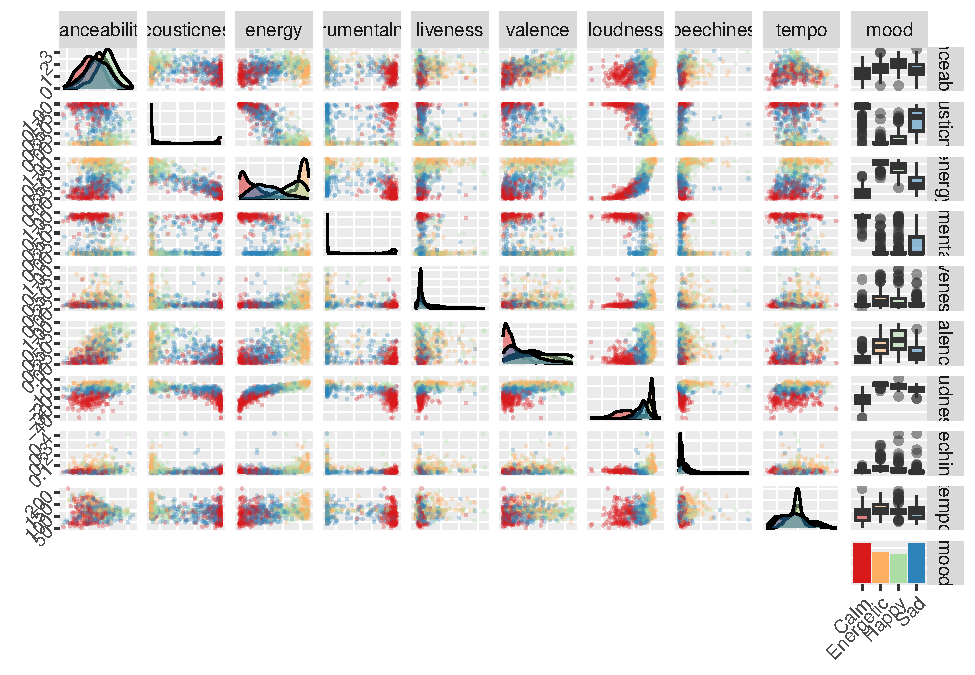
\includegraphics{figs/features} \caption{Features inspection with respect to each mood labeled.}\label{fig:features}
\end{figure}

Also, from the scatter plots appearing in \ref{fig:features}, we can see
that some of the variables are highly correlated. \ref{fig:cor} contains
the correlation matrix for the variables, presenting both negative and
positive correlation among some of the features, such as loudness with
energy (positive) and aciusticness with energy (negative).

\begin{figure}[H]
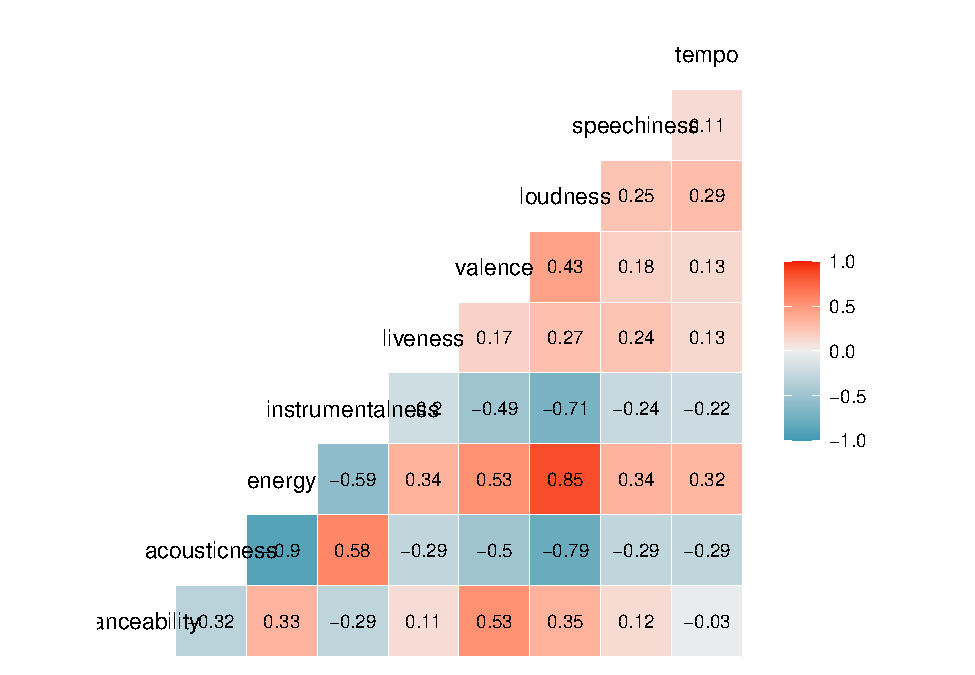
\includegraphics{figs/cor} \caption{Correlation plot of the features.}\label{fig:cor}
\end{figure}

If we inspect closer the distribution of moods in our dataset,
(Fig.\ref{fig:count}), we can see that our dataset is pretty balanced,
containing more than enough songs to characterize each mood.

\begin{figure}[H]
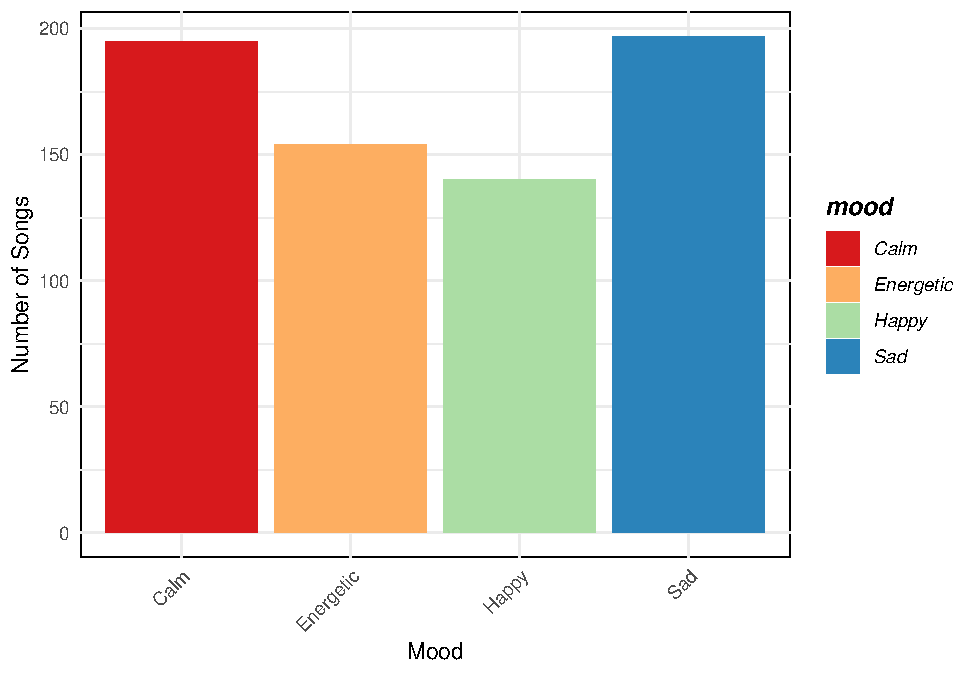
\includegraphics{figs/count} \caption{Histogram of the amount of songs classified in each emotion}\label{fig:count}
\end{figure}

Lastly, Fig \ref{fig:radar} shows a characterization of each of the
moods using a Radar plot. As you can see, calm songs are characterized
by being both heavily acoustic and instrumental, while happy songs are
highly danceable and energetic, being moderatelly loud. Sad songs seems
to be very valanced in every aspect except from speechiness and
energetic songs are characterized by being energetic and loud.

\begin{figure}[H]
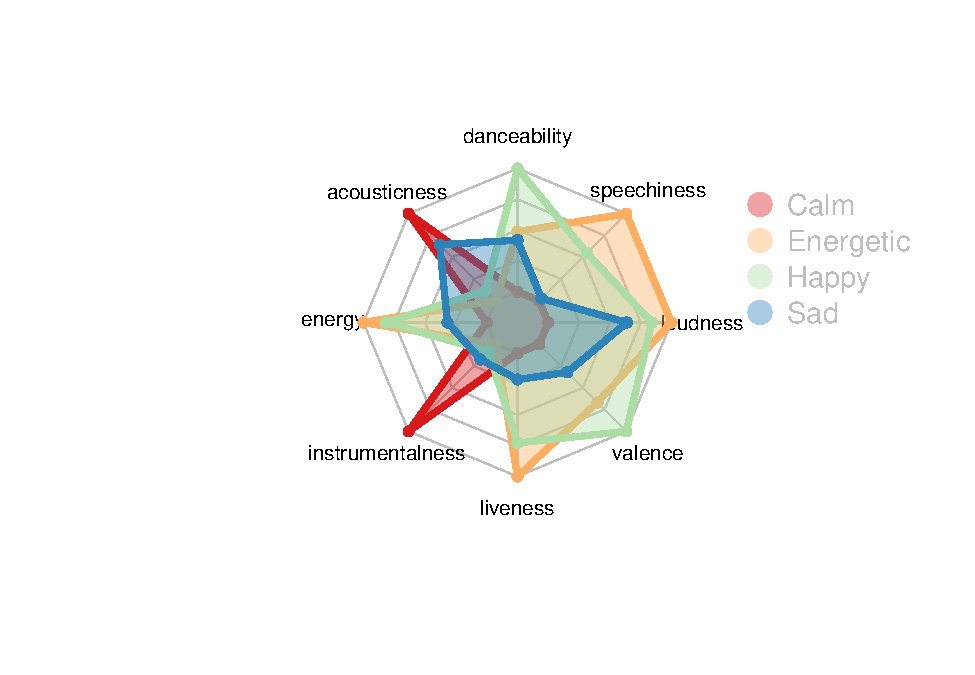
\includegraphics{figs/radar} \caption{Radar plot showcasing the average values of the features that characterize each of the moods}\label{fig:radar}
\end{figure}

\hypertarget{methodolody}{%
\section{Methodolody}\label{methodolody}}

To train our models, we have split our dataset into a training set
(80\%) and a test set (20\%). Shuffling is not necessary as the dataset
is not ordered. Our approach to finding the best model involves fitting
several models using all numerical features available in our dataset,
including `danceability', `acousticness', `energy', `instrumentalness',
`liveness', `valence', `loudness', `speechiness', and `tempo'.
Afterwards, we will select the best performing model and improve it
through feature selection and hyperparameter tuning. The model with the
highest performance will then be refitted with the entire dataset and
integrated into our Shiny app. To fit all the models, \texttt{caret}
package \citep{caret} will be used, 5-folds CV will be applied, and we
will center and scale the predictors.

\hypertarget{multinomial-logistic-regression}{%
\subsection{Multinomial Logistic
Regression}\label{multinomial-logistic-regression}}

We will begin by applying the most basic model, which is a logistic
regression. In this case, we will use a multinomial logistic regression
since our categories are not binary.

\begin{verbatim}
## Penalized Multinomial Regression 
## 
## 550 samples
##   9 predictor
##   4 classes: 'Calm', 'Energetic', 'Happy', 'Sad' 
## 
## Pre-processing: centered (9), scaled (9) 
## Resampling: Cross-Validated (5 fold) 
## Summary of sample sizes: 440, 440, 440, 439, 441 
## Resampling results across tuning parameters:
## 
##   decay  Accuracy   Kappa    
##   0e+00  0.7982580  0.7286732
##   1e-04  0.7982580  0.7286732
##   1e-01  0.7981922  0.7287540
## 
## Kappa was used to select the optimal model using the largest value.
## The final value used for the model was decay = 0.1.
\end{verbatim}

\begin{verbatim}
## Confusion Matrix and Statistics
## 
##            Reference
## Prediction  Calm Energetic Happy Sad
##   Calm        37         0     0   2
##   Energetic    0        23     8   0
##   Happy        0         7    17   2
##   Sad          2         0     3  35
## 
## Overall Statistics
##                                           
##                Accuracy : 0.8235          
##                  95% CI : (0.7489, 0.8835)
##     No Information Rate : 0.2868          
##     P-Value [Acc > NIR] : < 2.2e-16       
##                                           
##                   Kappa : 0.7627          
##                                           
##  Mcnemar's Test P-Value : NA              
## 
## Statistics by Class:
## 
##                      Class: Calm Class: Energetic Class: Happy Class: Sad
## Sensitivity               0.9487           0.7667       0.6071     0.8974
## Specificity               0.9794           0.9245       0.9167     0.9485
## Pos Pred Value            0.9487           0.7419       0.6538     0.8750
## Neg Pred Value            0.9794           0.9333       0.9000     0.9583
## Prevalence                0.2868           0.2206       0.2059     0.2868
## Detection Rate            0.2721           0.1691       0.1250     0.2574
## Detection Prevalence      0.2868           0.2279       0.1912     0.2941
## Balanced Accuracy         0.9640           0.8456       0.7619     0.9229
\end{verbatim}

Although multinomial logistic regression model appears to be effective
in classifying songs into their respective moods, with an accuracy of
\textasciitilde80\% and \(\kappa = 0.76\),we will keep trying more
appropriate methods for non-binary classification problems, such as LDA
for \(p>1\). Before that, lets have a look at the coefficients computed
for each variable

\begin{table}[!h]

\caption{\label{tab:unnamed-chunk-3}Coefficients for mood = Energetic}
\centering
\resizebox{\linewidth}{!}{
\begin{tabular}[t]{lrrrrrrrrrr}
\toprule
  & (Intercept) & danceability & acousticness & energy & instrumentalness & liveness & valence & loudness & speechiness & tempo\\
\midrule
\cellcolor{gray!6}{Coefficient} & \cellcolor{gray!6}{-1.8037649} & \cellcolor{gray!6}{0.5121807} & \cellcolor{gray!6}{-1.9035712} & \cellcolor{gray!6}{4.1097341} & \cellcolor{gray!6}{-4.4191853} & \cellcolor{gray!6}{0.6185421} & \cellcolor{gray!6}{1.1889409} & \cellcolor{gray!6}{3.4788527} & \cellcolor{gray!6}{-0.0894802} & \cellcolor{gray!6}{0.4523645}\\
Std. Errors & 1.0888229 & 0.4516770 & 0.8134856 & 1.1198090 & 0.6506191 & 0.6403064 & 0.5921362 & 1.1964151 & 0.6271437 & 0.4224320\\
\cellcolor{gray!6}{z stat} & \cellcolor{gray!6}{-1.6566192} & \cellcolor{gray!6}{1.1339536} & \cellcolor{gray!6}{-2.3400183} & \cellcolor{gray!6}{3.6700314} & \cellcolor{gray!6}{-6.7922767} & \cellcolor{gray!6}{0.9660095} & \cellcolor{gray!6}{2.0078844} & \cellcolor{gray!6}{2.9077304} & \cellcolor{gray!6}{-0.1426789} & \cellcolor{gray!6}{1.0708577}\\
p value & 0.0975965 & 0.2568140 & 0.0192828 & 0.0002425 & 0.0000000 & 0.3340394 & 0.0446556 & 0.0036406 & 0.8865438 & 0.2842334\\
\bottomrule
\end{tabular}}
\end{table}

\begin{table}[!h]

\caption{\label{tab:unnamed-chunk-3}Coefficients for mood = Happy}
\centering
\resizebox{\linewidth}{!}{
\begin{tabular}[t]{lrrrrrrrrrr}
\toprule
  & (Intercept) & danceability & acousticness & energy & instrumentalness & liveness & valence & loudness & speechiness & tempo\\
\midrule
\cellcolor{gray!6}{Coefficient} & \cellcolor{gray!6}{1.7063251} & \cellcolor{gray!6}{1.0854503} & \cellcolor{gray!6}{-1.3099355} & \cellcolor{gray!6}{3.123178} & \cellcolor{gray!6}{-3.4162837} & \cellcolor{gray!6}{0.5534468} & \cellcolor{gray!6}{1.6673193} & \cellcolor{gray!6}{0.9929464} & \cellcolor{gray!6}{-0.1377737} & \cellcolor{gray!6}{0.5614269}\\
Std. Errors & 0.7922969 & 0.4175990 & 0.5734972 & 1.015434 & 0.5739915 & 0.6304147 & 0.5733037 & 1.0095547 & 0.6175027 & 0.4023728\\
\cellcolor{gray!6}{z stat} & \cellcolor{gray!6}{2.1536436} & \cellcolor{gray!6}{2.5992650} & \cellcolor{gray!6}{-2.2841182} & \cellcolor{gray!6}{3.075708} & \cellcolor{gray!6}{-5.9518015} & \cellcolor{gray!6}{0.8779090} & \cellcolor{gray!6}{2.9082652} & \cellcolor{gray!6}{0.9835489} & \cellcolor{gray!6}{-0.2231144} & \cellcolor{gray!6}{1.3952904}\\
p value & 0.0312681 & 0.0093424 & 0.0223646 & 0.002100 & 0.0000000 & 0.3799931 & 0.0036344 & 0.3253374 & 0.8234465 & 0.1629283\\
\bottomrule
\end{tabular}}
\end{table}

\begin{table}[!h]

\caption{\label{tab:unnamed-chunk-3}Coefficients for mood = Sad}
\centering
\resizebox{\linewidth}{!}{
\begin{tabular}[t]{lrrrrrrrrrr}
\toprule
  & (Intercept) & danceability & acousticness & energy & instrumentalness & liveness & valence & loudness & speechiness & tempo\\
\midrule
\cellcolor{gray!6}{Coefficient} & \cellcolor{gray!6}{3.8190113} & \cellcolor{gray!6}{-0.1399674} & \cellcolor{gray!6}{-0.2790502} & \cellcolor{gray!6}{0.2507406} & \cellcolor{gray!6}{-2.7361226} & \cellcolor{gray!6}{0.2842616} & \cellcolor{gray!6}{1.2273135} & \cellcolor{gray!6}{2.0233308} & \cellcolor{gray!6}{-0.3899211} & \cellcolor{gray!6}{-0.1526533}\\
Std. Errors & 0.7077692 & 0.3288764 & 0.4355993 & 0.8415041 & 0.4808576 & 0.5943572 & 0.5285823 & 0.6882719 & 0.6016057 & 0.2987553\\
\cellcolor{gray!6}{z stat} & \cellcolor{gray!6}{5.3958429} & \cellcolor{gray!6}{-0.4255928} & \cellcolor{gray!6}{-0.6406121} & \cellcolor{gray!6}{0.2979672} & \cellcolor{gray!6}{-5.6900892} & \cellcolor{gray!6}{0.4782673} & \cellcolor{gray!6}{2.3218967} & \cellcolor{gray!6}{2.9397261} & \cellcolor{gray!6}{-0.6481340} & \cellcolor{gray!6}{-0.5109644}\\
p value & 0.0000001 & 0.6704046 & 0.5217748 & 0.7657282 & 0.0000000 & 0.6324600 & 0.0202385 & 0.0032850 & 0.5168983 & 0.6093760\\
\bottomrule
\end{tabular}}
\end{table}

As we can see in the tables above, some of the coefficients do not
affect the dependent variable. This is due to the multicolinearity found
before in Fig. \ref{fig:cor}.

\hypertarget{linear-discriminant-analysis-lda-p-1}{%
\subsection{Linear Discriminant Analysis (LDA, p \textgreater{}
1)}\label{linear-discriminant-analysis-lda-p-1}}

\begin{verbatim}
## Linear Discriminant Analysis 
## 
## 550 samples
##   9 predictor
##   4 classes: 'Calm', 'Energetic', 'Happy', 'Sad' 
## 
## Pre-processing: centered (9), scaled (9) 
## Resampling: Cross-Validated (5 fold) 
## Summary of sample sizes: 440, 440, 440, 439, 441 
## Resampling results:
## 
##   Accuracy   Kappa    
##   0.7745379  0.6975865
\end{verbatim}

\begin{verbatim}
## Confusion Matrix and Statistics
## 
##            Reference
## Prediction  Calm Energetic Happy Sad
##   Calm        36         0     0   2
##   Energetic    0        23    10   0
##   Happy        0         7    16   5
##   Sad          3         0     2  32
## 
## Overall Statistics
##                                           
##                Accuracy : 0.7868          
##                  95% CI : (0.7083, 0.8523)
##     No Information Rate : 0.2868          
##     P-Value [Acc > NIR] : < 2.2e-16       
##                                           
##                   Kappa : 0.7141          
##                                           
##  Mcnemar's Test P-Value : NA              
## 
## Statistics by Class:
## 
##                      Class: Calm Class: Energetic Class: Happy Class: Sad
## Sensitivity               0.9231           0.7667       0.5714     0.8205
## Specificity               0.9794           0.9057       0.8889     0.9485
## Pos Pred Value            0.9474           0.6970       0.5714     0.8649
## Neg Pred Value            0.9694           0.9320       0.8889     0.9293
## Prevalence                0.2868           0.2206       0.2059     0.2868
## Detection Rate            0.2647           0.1691       0.1176     0.2353
## Detection Prevalence      0.2794           0.2426       0.2059     0.2721
## Balanced Accuracy         0.9512           0.8362       0.7302     0.8845
\end{verbatim}

the LDA and logistic regression predictions are almost identical, as
Section 4.5 of \citep{book} discusses.

\hypertarget{quadratic-discriminant-analysis-qda}{%
\subsection{Quadratic Discriminant Analysis
(QDA)}\label{quadratic-discriminant-analysis-qda}}

\begin{verbatim}
## Quadratic Discriminant Analysis 
## 
## 550 samples
##   9 predictor
##   4 classes: 'Calm', 'Energetic', 'Happy', 'Sad' 
## 
## Pre-processing: centered (9), scaled (9) 
## Resampling: Cross-Validated (5 fold) 
## Summary of sample sizes: 440, 440, 440, 439, 441 
## Resampling results:
## 
##   Accuracy   Kappa    
##   0.7835961  0.7091766
\end{verbatim}

\begin{verbatim}
## Confusion Matrix and Statistics
## 
##            Reference
## Prediction  Calm Energetic Happy Sad
##   Calm        37         0     0   2
##   Energetic    0        20     9   0
##   Happy        0         9    16   4
##   Sad          2         1     3  33
## 
## Overall Statistics
##                                           
##                Accuracy : 0.7794          
##                  95% CI : (0.7003, 0.8459)
##     No Information Rate : 0.2868          
##     P-Value [Acc > NIR] : < 2.2e-16       
##                                           
##                   Kappa : 0.7037          
##                                           
##  Mcnemar's Test P-Value : NA              
## 
## Statistics by Class:
## 
##                      Class: Calm Class: Energetic Class: Happy Class: Sad
## Sensitivity               0.9487           0.6667       0.5714     0.8462
## Specificity               0.9794           0.9151       0.8796     0.9381
## Pos Pred Value            0.9487           0.6897       0.5517     0.8462
## Neg Pred Value            0.9794           0.9065       0.8879     0.9381
## Prevalence                0.2868           0.2206       0.2059     0.2868
## Detection Rate            0.2721           0.1471       0.1176     0.2426
## Detection Prevalence      0.2868           0.2132       0.2132     0.2868
## Balanced Accuracy         0.9640           0.7909       0.7255     0.8921
\end{verbatim}

Up to this point, the three models fitted seems to perform very
similarly on our dataset. To wrap up the model testing, we will fit try
Naive Bayes

\hypertarget{naive-bayes}{%
\subsection{Naive Bayes}\label{naive-bayes}}

\begin{verbatim}
## Naive Bayes 
## 
## 550 samples
##   9 predictor
##   4 classes: 'Calm', 'Energetic', 'Happy', 'Sad' 
## 
## Pre-processing: centered (9), scaled (9) 
## Resampling: Cross-Validated (5 fold) 
## Summary of sample sizes: 440, 440, 440, 439, 441 
## Resampling results across tuning parameters:
## 
##   usekernel  Accuracy   Kappa    
##   FALSE      0.7964065  0.7267479
##    TRUE      0.7818110  0.7076660
## 
## Tuning parameter 'fL' was held constant at a value of 0
## Tuning
##  parameter 'adjust' was held constant at a value of 1
## Kappa was used to select the optimal model using the largest value.
## The final values used for the model were fL = 0, usekernel = FALSE and adjust
##  = 1.
\end{verbatim}

\begin{verbatim}
## Confusion Matrix and Statistics
## 
##            Reference
## Prediction  Calm Energetic Happy Sad
##   Calm        35         0     0   2
##   Energetic    0        23    10   0
##   Happy        0         6    15   6
##   Sad          4         1     3  31
## 
## Overall Statistics
##                                           
##                Accuracy : 0.7647          
##                  95% CI : (0.6844, 0.8332)
##     No Information Rate : 0.2868          
##     P-Value [Acc > NIR] : < 2.2e-16       
##                                           
##                   Kappa : 0.6843          
##                                           
##  Mcnemar's Test P-Value : NA              
## 
## Statistics by Class:
## 
##                      Class: Calm Class: Energetic Class: Happy Class: Sad
## Sensitivity               0.8974           0.7667       0.5357     0.7949
## Specificity               0.9794           0.9057       0.8889     0.9175
## Pos Pred Value            0.9459           0.6970       0.5556     0.7949
## Neg Pred Value            0.9596           0.9320       0.8807     0.9175
## Prevalence                0.2868           0.2206       0.2059     0.2868
## Detection Rate            0.2574           0.1691       0.1103     0.2279
## Detection Prevalence      0.2721           0.2426       0.1985     0.2868
## Balanced Accuracy         0.9384           0.8362       0.7123     0.8562
\end{verbatim}

We can compare the four models applyied using \texttt{resamples}
function from the \texttt{caret} package \citep{caret}

\begin{figure}[H]
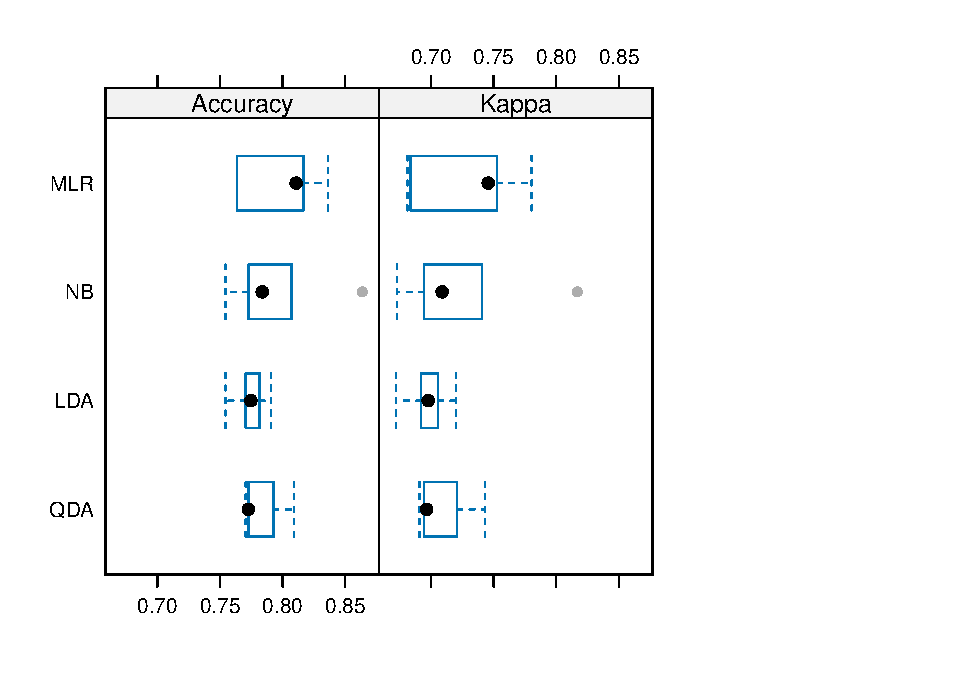
\includegraphics{figs/resamp} \caption{Resampling results using `resamples` function from the `caret` package [@caret] }\label{fig:resamp}
\end{figure}

The main results obtained from Fig. \ref{fig:resamp} can be summarized
as follows:

Accuracy:

\begin{itemize}
\tightlist
\item
  Logistic Regression (MLR): Mean accuracy of approximately \(79.82 \%\)
\item
  Linear Discriminant Analysis (LDA): Mean accuracy of approximately
  \(77.45 \%\)
\item
  Quadratic Discriminant Analysis (QDA): Mean accuracy of approximately
  \(78.36 \%\)
\item
  Naive Bayes (NB): Mean accuracy of approximately \(79.64 \%\)
\end{itemize}

Kappa:

\begin{itemize}
\tightlist
\item
  Logistic Regression (MLR): Mean Kappa of approximately 0.7288
\item
  Linear Discriminant Analysis (LDA): Mean Kappa of approximately 0.6976
\item
  Quadratic Discriminant Analysis (QDA): Mean Kappa of approximately
  0.7092
\item
  Naive Bayes (NB): Mean Kappa of approximately 0.7267
\end{itemize}

Based on these metrics, the logistic regression model (MLR) has the
highest mean accuracy and Kappa value among the four models. It is also
convenient in terms of interpretability and computational efficiency.
Therefore, the logistic regression model may be considered the best
model for this classification task.

\hypertarget{feature-selection-on-multinomial-linear-regression}{%
\subsection{Feature selection on Multinomial Linear
Regression}\label{feature-selection-on-multinomial-linear-regression}}

Lets apply BIC criterion to perform feature selection:

\begin{verbatim}
## Best model formula: ~ mood acousticness + energy + instrumentalness + liveness + valence + loudness
\end{verbatim}

\begin{verbatim}
## BIC: 608.8062
\end{verbatim}

\begin{figure}[H]
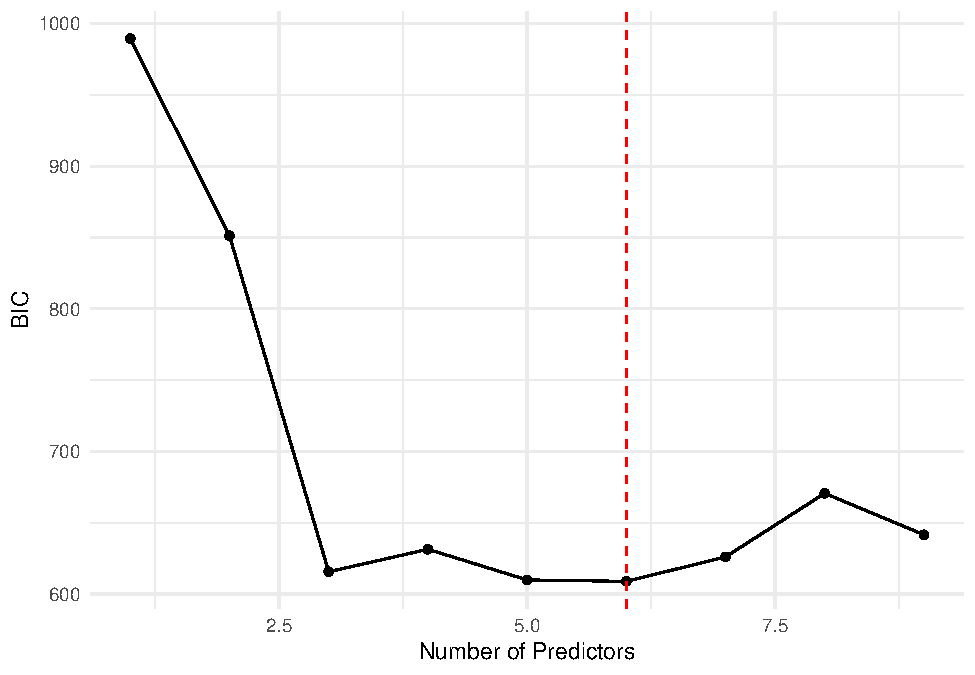
\includegraphics{figs/BIC} \caption{Evolution of BIC with Number of Predictors}\label{fig:BIC}
\end{figure}

The best model found, based in BIC criterion, is
\texttt{mood\ \textasciitilde{}\ acousticness\ +\ energy\ +\ instrumentalness\ +\ liveness\ +\ valence\ +\ loudness}
with a \$BIC = 608.80''. Fitting this model:

\begin{verbatim}
## Penalized Multinomial Regression 
## 
## 550 samples
##   6 predictor
##   4 classes: 'Calm', 'Energetic', 'Happy', 'Sad' 
## 
## Pre-processing: centered (6), scaled (6) 
## Resampling: Cross-Validated (5 fold) 
## Summary of sample sizes: 440, 440, 440, 439, 441 
## Resampling results across tuning parameters:
## 
##   decay  Accuracy   Kappa    
##   0e+00  0.7982580  0.7286534
##   1e-04  0.7982580  0.7286534
##   1e-01  0.8001089  0.7311467
## 
## Kappa was used to select the optimal model using the largest value.
## The final value used for the model was decay = 0.1.
\end{verbatim}

\begin{verbatim}
## Confusion Matrix and Statistics
## 
##            Reference
## Prediction  Calm Energetic Happy Sad
##   Calm        38         0     0   2
##   Energetic    0        24     9   0
##   Happy        0         5    17   2
##   Sad          1         1     2  35
## 
## Overall Statistics
##                                           
##                Accuracy : 0.8382          
##                  95% CI : (0.7654, 0.8958)
##     No Information Rate : 0.2868          
##     P-Value [Acc > NIR] : < 2.2e-16       
##                                           
##                   Kappa : 0.7824          
##                                           
##  Mcnemar's Test P-Value : NA              
## 
## Statistics by Class:
## 
##                      Class: Calm Class: Energetic Class: Happy Class: Sad
## Sensitivity               0.9744           0.8000       0.6071     0.8974
## Specificity               0.9794           0.9151       0.9352     0.9588
## Pos Pred Value            0.9500           0.7273       0.7083     0.8974
## Neg Pred Value            0.9896           0.9417       0.9018     0.9588
## Prevalence                0.2868           0.2206       0.2059     0.2868
## Detection Rate            0.2794           0.1765       0.1250     0.2574
## Detection Prevalence      0.2941           0.2426       0.1765     0.2868
## Balanced Accuracy         0.9769           0.8575       0.7712     0.9281
\end{verbatim}

In this case, since we want to increase the accuracy as much as possible
to improve the classification process, we will use all the predictors
available to fit the model. Thus, the final model used in our Shiny app
will be the following:

\begin{Shaded}
\begin{Highlighting}[]
\NormalTok{ctrl }\OtherTok{\textless{}{-}} \FunctionTok{trainControl}\NormalTok{(}\AttributeTok{method =} \StringTok{"cv"}\NormalTok{, }\AttributeTok{number =} \DecValTok{5}\NormalTok{,}
                     \AttributeTok{classProbs =} \ConstantTok{TRUE}\NormalTok{, }
                     \AttributeTok{verboseIter=}\ConstantTok{FALSE}\NormalTok{)}

\NormalTok{log.fit }\OtherTok{=} \FunctionTok{train}\NormalTok{(mood }\SpecialCharTok{\textasciitilde{}}\NormalTok{ acousticness }\SpecialCharTok{+}\NormalTok{ energy }\SpecialCharTok{+}\NormalTok{ instrumentalness }\SpecialCharTok{+}\NormalTok{ liveness }\SpecialCharTok{+}\NormalTok{ valence }\SpecialCharTok{+}\NormalTok{ loudness, }
               \AttributeTok{method =} \StringTok{"multinom"}\NormalTok{,}
               \AttributeTok{metric =} \StringTok{"Kappa"}\NormalTok{,}
               \AttributeTok{data =}\NormalTok{ numeric\_data,}
               \AttributeTok{preProcess =} \FunctionTok{c}\NormalTok{(}\StringTok{"center"}\NormalTok{, }\StringTok{"scale"}\NormalTok{),}
               \AttributeTok{trControl =}\NormalTok{ ctrl,}
               \AttributeTok{trace =} \ConstantTok{FALSE}\NormalTok{)}
\CommentTok{\# Save the trained model}
\FunctionTok{saveRDS}\NormalTok{(log.fit, }\StringTok{"trained\_model.rds"}\NormalTok{)}
\end{Highlighting}
\end{Shaded}

When applying in a future Machine Learning for classification, KNN is
expected to outperform LDA and logistic regression in cases where the
decision boundary is highly non-linear, given a large n and small p,
because KNN is non-parametric. However, accurate classification with KNN
requires a substantial number of observations relative to the number of
predictors, meaning that n must be much larger. The non-parametric
nature of KNN reduces bias but incurs a high level of variance, which
can result in a decision boundary that is non-linear when n is moderate
or p is not very small. In such situations, QDA may be a more suitable
option than KNN as it can provide a non-linear decision boundary while
taking advantage of a parametric form. This results in a smaller
required sample size for accurate classification compared to KNN.

\hypertarget{shiny-app}{%
\section{Shiny app}\label{shiny-app}}

\hypertarget{references}{%
\section{References}\label{references}}

\setlength{\parindent}{-0.2in}
\setlength{\leftskip}{0.2in}
\setlength{\parskip}{8pt}
\vspace*{-0.2in}

\noindent





\newpage
\singlespacing
\bibliography{master.bib}

\end{document}
